\documentclass[12pt]{article}
\usepackage{sbc-template} 
\usepackage{graphicx,url}
\usepackage{url}
\usepackage[brazil]{babel} 
\usepackage[utf8]{inputenc} 
\usepackage[T1]{fontenc}
\usepackage[normalem]{ulem}
\usepackage[hidelinks]{hyperref}

\usepackage[square,authoryear]{natbib}
\usepackage{amssymb} 
\usepackage{mathalfa} 
\usepackage{algorithm} 
\usepackage{algpseudocode} 
\usepackage[table]{xcolor}
\usepackage{array}
\usepackage{titlesec}
\usepackage{mdframed}
\usepackage{listings}

\usepackage{amsmath} 
\usepackage{booktabs}

\urlstyle{same}

\newcolumntype{L}[1]{>{\raggedright\let\newline\\\arraybackslash\hspace{0pt}}m{#1}}
\newcolumntype{C}[1]{>{\centering\let\newline\\\arraybackslash\hspace{0pt}}m{#1}}
\newcolumntype{R}[1]{>{\raggedleft\let\newline\\\arraybackslash\hspace{0pt}}m{#1}}

\newcommand\Tstrut{\rule{0pt}{2.6ex}} 
\newcommand\Bstrut{\rule[-0.9ex]{0pt}{0pt}} 
\newcommand{\scell}[2][c]{\begin{tabular}[#1]{@{}c@{}}#2\end{tabular}}

\usepackage[nolist,nohyperlinks]{acronym}

\title{Anomaly Detection of Pump-and-Dump Schemes in Cryptocurrency Markets}

\author{Matheus Moura\inst{1}}


\address{Centro Federal de Educação Tecnológica Celso Suckow da Fonseca - CEFET/RJ
	\email{matheus.moura@aluno.cefet-rj.br}
}



\begin{document} 
	
	\maketitle
	
	\begin{resumo} 
		Este roteiro traz as principais informações para a elaboração de trabalhos científicos. o trabalho deve ser escrito de modo a se mostrar interessante e importante. Para tanto, a forma de escrevê-lo, principalmente no resumo e  introdução, é fundamental. É o momento no qual o autor deve ``vender o trabalho''. 
		
		Em textos científicos, as frases devem ser curtas, para não gerar ambiguidade. Pode-se dizer que um parágrafo é constituído por pelo menos três frases. Adicionalmente, pode-se dizer que cada parágrafo tem uma única ideia central, \emph{i.e.}, uma sentença  que sumariza o parágrafo. 
		
		O texto de um trabalho todo precisa estar encadeado \citep{zobel_writing_2015}. O encadeamento dos parágrafos é feito a partir do encadeamento de suas ideias centrais. Desta forma, a ideia central de cada parágrafo leva a ideia central do próximo e assim por diante. 
		
		Em linhas gerais, qualquer parágrafo do trabalho que não apresente citação é considerado criação dos autores. A utilização de textos transcritos de alguma fonte sem a devida referência a esta fonte e seus autores pode configurar a hipótese de plágio. Assim, todas as obras citadas devem ter as referências aos seus autores e devem figurar na lista de referências do trabalho.
	\end{resumo}
	
	\section{Introduction}
	\label{sec_introducao}

	The adoption of cryptocurrencies has experienced significant growth over the past decade, leading to a substantial expansion of the market both within traditional financial sectors and in public perception.
	This trend is exemplified by notable milestones, such as the approval of the first Bitcoin futures Exchange-traded fund (ETF) by the U.S. Securities and Exchange Commission (SEC) in 2021 \citep{wursthorn2021} and the trading commencement of spot ETFs on American stock exchanges in early 2024 \citep{schmitt2024}.
	The surge in public interest can be attributed to the exponential growth observed in the cryptocurrency market during late 2017 and early 2018, which captured widespread attention from mainstream media, attention that recurs with each subsequent occurrence of high bullish market trends \citep{steinmetz2021}.
	Consequently, there is a pressing need for comprehensive studies to assess the risks associated with this fairly new asset class.

	The vast majority of cryptocurrencies operate without reliance on any central authority and offer a degree of anonymity.
	These features facilitate their utilization in illicit activities, including but not limited to money laundering, drug trafficking, and hacking \citep{Kethineni2019}.
	Among the various fraudulent practices associated with cryptocurrencies, one prominent scheme is the pump-and-dump (P\&D) scheme, characterized by the artificial inflation of an asset's price followed by the sale of the acquired assets at a higher price \citep{li2021}.

	Organizers of pump-and-dumps leverage on social media platforms that offer some level of anonimity, such as Telegram and Discord.
	Where they establish a public group or channel and recruit as many members as possible for what are colloquially termed "pump groups".
	Within these groups only scheme organizers are allowed publishing messages and once a critical mass of members is attained, typically exceeding 1,000, operations commence \citep{xu2019}.

	The typical modus operandi of these groups starts with the dissemination of precise details, including the exact date, time, and exchange where the pump-and-dump operation will occur, allowing members adequate time to prepare their funds.
	At the pre-arranged time, the group administrators announce the targeted cryptocurrency and encourage members to acquire and retain it to artificially inflate its price.
	Throughout the pumping phase, participants promote the targeted coin on social media platforms to attract external attention.
	However, in a few minutes the price peak is reached and the participants begin panic-selling at the first sign of decline, leading to a rapid return of the coin's price to its pre-pump level \citep{xu2019}.

	Therefore, the detection of pump-and-dump holds significance in mitigating victimization and aiding market participants in identifying and addressing this kind of market manipulation.
	Pump-and-dump schemes manifest as anomalies within the time series data of the targeted cryptocurrency's price.
	This study investigates model deviation detection methods, a widely employed strategy for anomaly identification.
	This approach involves identifying events where there is a discrepancy between the observed behavior of the time series and the anticipated behavior as forecasted by a model \citep{ogasawara2024}.
	In contrast, our results are compared with that of \citet{lamorgia2020}, who employed a classification method for anomaly detection.

	\# Which approach was used in this work and how well it performed. (contributions)

	\# Work structure. 
	
	\section{Background}
	\label{sec_fund_teorica}

	The pump-and-dump scheme has a long history in the stock market \citep{lamorgia2020}.
	The subsequent subsection, Pump-and-Dump on Traditional Stock Market (see Subsection \ref{subsec_pump_def}) examines its operation within traditional stock markets.
	Following this examination, the subsection Pump-and-Dump on Cryptocurrency Markets (see Subsection \ref{subsec_pump_in_crypto}) explains why cryptocurrency markets are susceptible to the scheme and how the scheme has been adapted.
	By the end of this section, the subsection Cryptocurrency Pump-and-Dump as Time Series Anomalies (see Subsection \ref{subsec_pump_as_anomalies}) demonstrates the modeling of pump-and-dumps as anomalies within time series data and proposes methodologies for their detection.

	\subsection{Pump-and-Dump on Traditional Stock Market}
	\label{subsec_pump_def}

	The pump-and-dump scheme operates on a straightforward premise.
	Initially, the perpetrators identify a publicly traded security, typically of small size and with low trading volumes, as their target.
	Subsequently, they accumulate significant quantities of this security.
	Following acquisition, they start tounting the security, disseminating false and misleading information aimed at artificially inflating its price \citep{kramer2005}.

	Since the rise of the internet, anyone has been able to reach mass audiences, which created this new age of decentralized information.
	Concurrently, internet has facilitated the propagation of fraudulent activities reliant on information dissemination, which can now spread through various channels such as social media platforms, investment research websites, investment newsletters, online advertisements, and others.
	An early example of the pump-and-dump scheme's adaptation to the stock market using the internet occurred with the emergence of the website Fast-Trades.com in 1999.

	Fast-Trades operated as a stock selection website, providing recommendations to its subscribers while employing a six-month trial period to attract new users.
	The modus operandi was straightforward: the website owner and his friends initiated stock purchases prior to their disclosure as selections, concurrently placing sell limit orders\footnote{In this kind of order you set the lowest amount you would be willing to accept for each share you sell.}.
	Through this strategy, the perpetrators were able to profit several times the purchase price.
	For instance, their inaugural selection, Apache Medical Systems, saw its price surge to 600\% above the rate at which the site owner had purchased \citep{kramer2005}.

	During that time, the internet was a novel frontier, affording Fast-Trades.com perpetrators the opportunity to orchestrate the pump-and-dump scheme with minimal expertise in the stock market.
	Nevertheless, despite the internet's enabling role, it did not guarantee anonymity in their trades, as the stock market operates under centralized authorities with monitoring capabilities, which enabled regulators to uncover the scheme \citep{kramer2005}.
	Thus, the online fraudsters found themselves navigating a landscape where they possessed a potent means of reaching mass audiences, yet were constrained to operating within centralized and regulated markets.
	
	\subsection{Pump-and-Dump on Cryptocurrency Markets}
	\label{subsec_pump_in_crypto}

	This landscape was changed by \citet{nakamoto2008} with the introduction of Bitcoin and subsequent cryptocurrencies.
	Unlike traditional financial systems, the vast majority of cryptocurrencies operate without central authorities to process transactions, instead utilizing the peer-to-peer technology known as blockchain.
	This egalitarian nature of cryptocurrencies has ushered in a new era of decentralized authority, often affording privacy of transactions, dissociative anonymity, and a lack of deterrence \citep{Kethineni2019}.
	The convergence of these characteristics with the capabilities offered by the internet created a breakthrough, enabling online criminal activities such as the pump-and-dump scheme to proliferate with even more freedom.

	In cryptocurrency markets, the standard procedure for a pump-and-dump scheme commences with fraudsters establishing a publicly accessible group and recruiting a large number of participants.
	These groups often gravitate towards applications that offer encryption and anonymity features, with the majority being created on platforms such as Telegram or Discord.
	Additionally, the fraudsters typically configure these groups to restrict message publication solely to themselves, thereby minimizing potential interference from members.
	Once the group attain around 1,000 members the fraudsters can start operating the scheme \citep{xu2019}.

	The pump-and-dump operation commences with the announcement of the upcoming pump, typically occurring just a few days in advance.
	The fraudsters disclose the exchange\footnote{An organized market or center for trading cryptocurrencies.} where the pump will take place, the pairing coin\footnote{Cryptocurrency used trade against another cryptocurrency.} to be involved, and the precise date and time of the event.
	This advance notice allows members to make necessary preparations beforehand \citep{xu2019}.

	As the pump event draws near, the fraudsters disseminate countdowns and offer guidance, advising participants to swiftly execute purchases, subsequently promoting the coin to attract external investors, and emphasizing the importance of not selling below the current price.
	Concurrently, they leverage historical profit examples to incentivize members participation.
	Upon the predetermined time's arrival, the fraudsters announce the targeted coin and urge members to buy and hold it to artificially inflate its price \citep{xu2019}.

	The pump typically culminates in a peak price within a few minutes of initiation.
	Subsequently, at the first sign of price decline, all participants commence panic-selling the coin.
	Within approximately half an hour, the cryptocurrency retraces to its pre-pump price and trading volume.
	After that, the fraudsters release a review of the pump, cherry-picking data that supports the hypothesis of high profitability for scheme participants \citep{xu2019}.

	Hence, a fundamental characteristic of pump-and-dump schemes within cryptocurrency markets is the establishment of publicly accessible groups, where every member is aware of the scheme.
	The reason for participation stems from the promise of quick and substantial profits.
	Additionally, group members are consider that individuals who join the pump through their social media advertisements are the scheme's victims, and their own profitability hinges only on how fast they are operating.
	However, as shown by \citet{xu2019}, the majority of members ultimately fall victim to the scheme, purchasing at an already inflated price, while the orchestrators, who initiate buy and sell orders prior to the pump, enjoy almost guaranteed profits.

	\subsection{Cryptocurrency Pump-and-Dump as Time Series Anomalies}
	\label{subsec_pump_as_anomalies}

	The ultimate goal of a pump-and-dump scheme in cryptocurrency markets is to artificially inflate the price of a coin for profit.
	However, due to the brief duration during which they can sustain the inflated price, the impact of such schemes on the price time series of the targeted coin is often perceived as a point anomaly.
	Anomaly detection constitutes a significant area of study within event detection literature, with certain methods already explored for detecting pump-and-dumps in cryptocurrency markets.

	Two prominent studies have expored anomaly detection methodologies for cryptocurrency pump-and-dumps.
	The first, conducted by \citet{kamps2018}, emphasized the utilization of unsupervised anomaly detection techniques, prompted by the scarcity of labeled data available at the time.
	Addressing this challenge, \citet{lamorgia2020} contributed with a public labeled dataset, along with the implementation of classification-based anomaly detection methods that demonstrated a great improvement in results compared to \citet{kamps2018} detector.

	\section{Related Work}
	\label{sec_trab_relacionados}

	The research conducted by \citet{kamps2018} was one of the pioneering studies in the field of cryptocurrency pump-and-dump schemes.
	It offered an initial formalization of these schemes and proposed a methodology for detecting them using anomaly detection algorithms.
	Given the nature of pump-and-dump schemes and the limited availability of labeled data at the time, they come up with a detector for local anomalies based on unsupervised anomaly detection algorithms, focusing on recent historical data.

	\citet{kamps2018} detector utilizes candlesticks with hourly intervals, incorporating data on open, highest, lowest, and close prices and volumes.
	Their approach employs two anomaly thresholds based on transaction volume and coin price.
	Events exceeding both thresholds are identified as pump-and-dump schemes.
	Additionally, they proposed three threshold calculation configurations aimed at maximizing recall, maximizing precision, and balancing both metrics.
	However, their study lacked established metrics due to the absence of ground truth in the dataset utilized.

	In contrast, \citet{lamorgia2020} conducted a study centered on pump-and-dump activities operated by the group Big Pump Signal which mainly operated within the Binance exchange, representing the largest group identified by them.
	One of their key contributions is a labeled dataset derived from pump-and-dump schemes operated on the Binance exchange by the monitored groups.
	The dataset was created utilizing the Binance API, enabling retrieval of every transaction within the complete trading pair history.

	Another notable contribution of \citet{lamorgia2020} study is the development of an anomaly detection algorithm based on classification methods.
	They analyze various types of features and utilize them as inputs for two distinct classifiers: Random Forest and Logistic Regression.
	Furthermore, they present results for intervals of 5, 15, and 25 seconds of aggregated orders.
	In the end, they conduct a comparative analysis with \citet{kamps2018}, applying their methodology to the dataset and demonstrating a notable enhancement in the F1 metric, from 60.5\% to 92.0\%, which are further explored in Section \ref{sec_aval_exp}.

	
	\section{Method}
	\label{sec_metodo}

	The methodology section in this work covers the whole workflow applied to the data for the anomaly detection and is defined according to Figure \ref{fig_metodology_flow}.
	It can be summarized in the following steps:
	    Orders History Dataset (See Subsection \ref{subsec_met_dataset});
	    Data Enrichment (See Subsection \ref{subsec_met_enrichment});
	    Data Preprocessing (See Subsection \ref{subsec_met_preprocessing});
	    Anomaly Detection (See Subsection \ref{subsec_met_anomaly_detection}).
	These steps are described in detail in the following subsections.

	\begin{figure}[!ht]
		\centering
		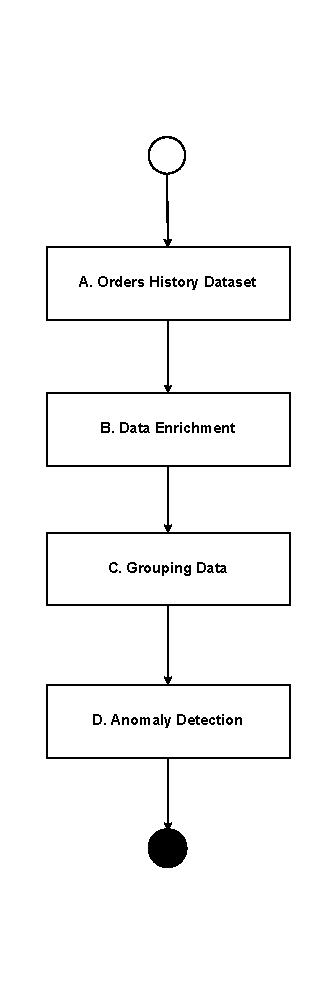
\includegraphics[scale=0.8]{figures/met-flow.pdf}
		\caption{Data analytics workflow for anomaly detection}
		\label{fig_metodology_flow}
	\end{figure}

    \subsection{Orders History Dataset}
	\label{subsec_met_dataset}

    Constructing a dataset of pump-and-dump events is a formidable challenge, necessitating longitudinal monitoring of the groups perpetrating the scheme.
    To address this obstacle, the present study leverages datasets provided by \citet{lamorgia2020}.
    Consequently, our investigation is centered on pump-and-dump occurrences within the Binance exchange.
    By utilizing their resources, we acquired 339 datasets pertaining to Binance pump-and-dump events.

    Each dataset has 14 days of historical trading data, encompassing 7 days prior to and 7 days following the event under analysis.
    The dataset consists of trade records, including volume in Bitcoin, quantity, price, operation type (buy or sell), and UNIX timestamps.
    A sample of the data is provided in Table \ref{tab_dataset_sample}.

    \begin{table}[!ht]
        \centering
        \caption{Sample of historical trading data obtained from Binance API}
        \begin{tabular}{cccccc}
            \toprule
            \textbf{Pair Symbol} & \textbf{Timestamp} & \textbf{Side} & \textbf{Price} & \textbf{Amount} & \textbf{Volume (BTC)} \\
            \midrule
            YOYOW/BTC & 1603217086 & SELL & 5.5e-07 & 1000 & 0.00055 \\
            YOYOW/BTC & 1603217452 & BUY & 5.6e-07 & 48072 & 0.02692032 \\
            YOYOW/BTC & 1603219189 & SELL & 5.6e-07 & 185383 & 0.10381448 \\
            \bottomrule
        \end{tabular}
        \label{tab_dataset_sample}
    \end{table}

    However, it is noteworthy that the Binance API does not provide information regarding the type of order, such as Market, Limit, or Stop Loss.
    Additionally, a limitation of the dataset is that the cryptocurrency is paired with Bitcoin, rendering the data susceptible to fluctuations in the price of Bitcoin at the time of trading.
    Therefore, it is important to mitigate the impact of this variability before conducting analyses utilizing price data.

    \subsection{Data Enrichment}
	\label{subsec_met_enrichment}

    To address the potential impact of Bitcoin price volatility on our analysis, we augmented our methodology by integrating data from the Live Coin Watch API\footnote{\url{https://www.livecoinwatch.com/tools/api}} to retrieve the Bitcoin price at the time of order creation.
    With their API, we are able to access the price history spanning the last 8 years, with a time resolution of 15 minutes, which is enough for our analysis.
    Specifically, we queried the API for the Bitcoin/US dollar pair throughout the duration of each dataset, enabling us to infer the price of the cryptocurrency in US dollars.

    \subsection{Data Preprocessing}
	\label{subsec_met_preprocessing}
	
	Our preprocessing consists mainly into transforming the historical trading data into time series.
    The first stage of preprocessing is separate only the buy orders due to our main ideia of detect abnormal behavior of the buy orders.
    Subsequently, we aggregate the US dollar price for each order using the data obtained in the Data Enrichment process (See Subsection \ref{subsec_met_enrichment}).

    In the third stage, orders are aggregated into bins of an arbitrary number of seconds, a parameter of the method.
    Subsequently, for each aggregation of orders, key metrics constituting the time series, such as average US dollar price, number of orders, and total volume in US dollars, are computed.
    Finally, a label column is appended, indicating the bin in which the pump-and-dump event occurred.
    This process yields the dataset illustrated in Table \ref{tab_timeseries}.

    \begin{table}[!ht]
        \centering
        \caption{Example of time series after preprocessing}
        \begin{tabular}{cccccc}
            \toprule
            \textbf{Datetime} & \textbf{Average Price} & \textbf{Volume} & \textbf{Orders} & \textbf{Event} \\
            \midrule
            2020-10-20 18:10:52 & 0.00666 & 198.069 & 34 & FALSE \\
            2020-10-20 19:10:52 & 0.00666 & 180.427 & 29 & FALSE \\
            2020-10-20 20:10:52 & 0.00778 & 320.316 & 71 & TRUE \\
            \bottomrule
        \end{tabular}
        \label{tab_timeseries}
    \end{table}

    \subsection{Anomaly Detection}
	\label{subsec_met_anomaly_detection}

    Now that the time series has been generated, we can proceed to employ time series anomaly detection methods.
    In the context of this study, the models under investigation include ARIMA, GARCH, RED, and REMD.
    Each series is subjected to all models to identify anomalies, and the detection efficacy is evaluated utilizing the label column.

    Furthermore, the models are also evaluated using soft metrics.
    This approach is adopted due to the nature of each dataset, which pertains to a single pump-and-dump event.
    When employing hard metrics, the potential outcomes are limited to binary values of 0 or 1 for true positives.
    This aspect penalizes models that are inaccurate in identifying the exact event bin.
    Conversely, these models often exhibit fewer false positives.
    Therefore, using soft metrics allow for an evaluation of whether a model can detect the event, even if not precisely at the moment of occurrence.
	
	\section{Results and Discussion}
	\label{sec_aval_exp}

	This section presents the obtained results and discusses their impact.
	In order to facilitate the understanding of this section, we divided it into 4 subsections.
	The first subsection (\ref{subsec_exp_hyperparams}), outlines the hyperparameters used in the experiments.
	The second subsection (\ref{subsec_result_series_evals}) presents the results of the analysis conducted using the entire historical data for each event, spanning seven days before and seven days after.
	In the third subsection (\ref{subsec_result_time_interval}), we discuss the impact of different chunk sizes used for aggregating order history on the quality of the results.
	Finally, the last subsection (\ref{subsec_result_comparing}) compares the findings with the current state-of-the-art.

	\subsection{Hyperparameters Overview}
	\label{subsec_exp_hyperparams}
	
	There are two hyperparameters that influence our experiment.
	Firstly, the timeframe of order history analyzed, which has data from seven days before to seven days after the event.
	However, utilizing the entire history may not be the best scenario.
	While it provides more data, it still has only one labeled event so it also increases the likelihood of false positives.

	Another important hyperparameter is the chunk size, which determines the time window used to aggregate orders when constructing the time series.
	This parameter directly influences the quality of the results, as it defines the temporal resolution of the time series employed in the subsequent analysis.
	Besides that, the chunk size is also influenced by the size of the timeframe of order history because it some models require at least 100 observations in the time series.

	\subsection{Comprehensive Time Series Analysis}
	\label{subsec_result_series_evals}
	
	A avaliação experimental compreende uma avaliação quantitativa ou qualitativa do trabalho a partir de critérios estabelecidos para comparação.

	\subsection{Impact of Chunk Sizes on Analysis Quality}
	\label{subsec_result_time_interval}

	Como em qualquer experimento, a capacidade de reprodução é fundamental para sua validade.
	Sendo assim, é importante descrever o processo de experimentação adotados, apresentar os resultados propriamente dito, com uma síntese explicativa dos principais resultados.

	\subsection{Comparative Analysis}
	\label{subsec_result_comparing}
	Finalmente, devem ser apresentadas as ameaças ao estudo, \emph{i.e.}, qualquer coisa que possa tirar ou limitar a validade do experimento conduzido.

	\begin{table}[!ht]
        \centering
        \caption{Comparative of Best F1 methods}
        \begin{tabular}{lccccc}
            \toprule
            \textbf{Classifier} & \textbf{Chunk size} & \textbf{Precision} & \textbf{Recall} & \textbf{F1} \\
            \midrule
            Kamps (Strict) & 1 Hour & 50.1\% & 75.0\% & 60.5\% \\
            La Morgia (RF 10 Folds) & 25 Sec & 93.1\% & 91.4\% & 92.0\% \\
            ARIMA & 300 Sec & 2.86\% & 61.83\% & 2.90\% \\
            \bottomrule
        \end{tabular}
        \label{tab_comparison}
    \end{table}
	
	\section{Conclusion}
	\label{sec_conclusao}
	
	A conclusão é a finalização do trabalho e indica as conclusões obtidas com o desenvolvimento do trabalho, sejam elas positivas ou negativas. Nas conclusões, analisa-se o que era desejado (definido na introdução com os objetivos), comparando com o alcançado pelo trabalho, descrevendo como os objetivos foram alcançados e o porquê de algum objetivo não ter sido alcançado. Destacam-se também as contribuições do trabalho, incluindo os benefícios e inovações trazidas pelo trabalho.
	
	Apresentam-se os pontos do trabalho que merecem um maior aprofundamento de estudos. Isso possibilita a criação de novos trabalhos com estudos nesses pontos apresentados, na forma de uma continuidade das pesquisas efetuadas pelo trabalho. Os trabalhos futuros indicam, ainda, uma maturidade de pesquisa do autor do trabalho e esses pontos podem ser trabalhados, posteriormente.
	
	\section*{Acknowledgment}
	The authors thank the support provided by CAPES through the "Portal de Periódicos", which facilitated access to valuable resources for this research.
	
    \bibliographystyle{apalike}
	\bibliography{references}
	
\end{document}
